\documentclass{article}
\usepackage{graphicx} % Required for inserting images
\usepackage{blindtext}
\usepackage{graphicx}
\usepackage{mathtools}
\usepackage[a4paper, total={6in, 8in}]{geometry}

\begin{document}

\title{Evaluating the Determinants of Housing Prices}
\author{Aryan Arora and Muno Siyakurima}
\date{3/10/2022}

\maketitle

\noindent \emph{I am grateful to my coauthor for their support in checking over my R code and their contributions toward constructing our final model. I was solely responsible for this writeup so the quality of writing including all errors is strictly my own.}

\begin{center}
    \textbf{Abstract}
\end{center}

\noindent This paper seeks to estimate the effect of common home-value determinants like age, location, and size on average home values for California homes in 1990.\footnote{Homes refer to homes, apartments, duplexes, or any other residential unit} We construct a multiple regression model that identifies the impact that ocean proximity, housing median age, median income, total number of rooms in census block, and total number of bedrooms in its census block had on the value of California homes in 1990. We find that being farther from the ocean and a greater total number of rooms in a census block had a negative average effect on the mean home value, while ocean proximity and a higher median neighborhood income had a positive average effect on mean home values.\footnote{Home values in this dataset are occupant-reported by 1990 census respondents}

\section*{Introduction}

Individuals consider many factors when buying a home and not all factors are weighed equally. Yet, despite the subjective nature of home purchases, housing markets are often successful at finding market clearing prices for properties—reflecting a common valuation metric. This paper presents a multiple regression model for estimating the effect of determinants of home prices in California in 1990. We are investigating how factors such as proximity to the ocean or the total number of bedrooms in a census block, acting as a proxy for residential density, alter home values, holding all else equal. While this dataset is only applicable to California homes surveyed in 1990 and thus cannot predict housing prices today, it can help us better understand the California housing market in 1990. Additionally, the property value determinants that are shown to increase home values in 1990 likely continue to contribute positively to home values today—even if the degree to which they do so has likely changed. 

\section*{Data}

Our data was collected from the 1990 California Census data and was edited by Luis Torgo from the University of Porto. The data contains one row per census block group. A block typically contains between 600 and 3000 people (the mean number of people in a block in this sample is 1425.5 people). There were some modifications made to this dataset before we began to work with it. All census blocks which had a value of 0 for any of the included variables were dropped. Additionally, an ocean proximity variable was added which identified whether the specified block was close to the ocean, the bay, inland, or on an island. There were 207 values randomly removed from the total\_bedrooms column. We were not able to find any explanation of why they were removed. Furthermore, many median household values that are marked as \$500,001 in the dataset. We suspect that this has to do with how census data was collected in 1990. In 1990 the average price of a home was \$73,300, so a price above \$500,000 was extremely high (Demographia). We imagine that when responding to the Census survey, many respondents marked a box stating that their home value was ``Above \$500,000" and such responses were recorded as \$500,001. We modified the variable medianHouseValue by dividing all values by \$100,000. In our updated dataset medianHouseValue is measured in hundreds of thousands of dollars. Finally, we removed all rows containing missing data values. This resulted in 20,433 observations of 9 variables. Those 9 variables are:


\begin{table}[h]
\begin{tabular}{|l|p{0.75\linewidth}|}
\hline
\textbf{Variable Name:} & \textbf{Description:}                                            \\ \hline
longitude                               & A measure at how far east or west a home is. A larger value is farther west.    \\ \hline
latitude                                & A measure of how far north or south a home is. A larger value is farther north. \\ \hline
housingMedianAge & A measure of the median age of a home in a census block group. The larger the value, the older the median home is.                                      \\ \hline
totalRooms                              & A measure of the total number of rooms within a block group.                         \\ \hline
totalBedrooms                           & A measure of the total number of bedrooms within a block group.                      \\ \hline
population                              & A measure of the total number of people living within a block group.                 \\ \hline
households       & A measure of the total number of households in a block group. A household is defined as a group of people living within one home unit.        \\ \hline
medianIncome     & A measure of the median income for households within a block group. This is income on a household level and is measured in tens of thousands of dollars.     \\ \hline
medianHouseValue & The median value of a household within the block group. This variable is measured in hundreds of thousands of dollars.                                                        \\ \hline
oceanProximity   & This is a categorical variable that categorizes homes into five categories: Near Bay, Inland, \textless 1 Hour Ocean, Island, and Near Ocean. \\ \hline
\end{tabular}
\end{table}

\noindent  Note that home values, age, and income in our dataset are reported as the median values for census block groups. While this is limits the number of outliers we have to deal with, it biases our estimates. We are really measuring the mean of the median home value, age, and income which is an imperfect proxy for the mean. 

\section*{Results}

Our multiple regression model included all predictors in the dataset except latitude and longitude and included an interaction between log(population) and log(household). While all predictors appeared to be significant, we did not think it made rational sense for there to be a linear relationship between either latitude and longitude and the mean of the median housing prices.\footnote{While this is a statistics course, we are econometricians at heart and so we cannot, in good conscience, include a variable for which we can think of no theory to validate} Our model takes the following form: 

\begin{align*}
\mathrm{medianHouseValue} = \beta_{0}
    &+ \beta_{1}  \mathrm{oceanProximity} \\
    &+ \beta_{2}  \mathrm{housingMedianAge} \\
    &+ \beta_{3}  \mathrm{log(medianIncome)} \\
    &+ \beta_{4}  \mathrm{log(totalRooms)} \\
    &+ \beta_{5}  \mathrm{log(totalBedrooms)} \\
    &+ \beta_{6}  \mathrm{log(population)}  \\
    &+ \beta_{7}  \mathrm{log(households)}  \\
    &+ \beta_{8}  \mathrm{log(population) \times log(households)} + \epsilon\\
\end{align*}
\setlength\parindent{0pt}



Our model produced the following coefficient estimates and standard errors:

\begin{center}
    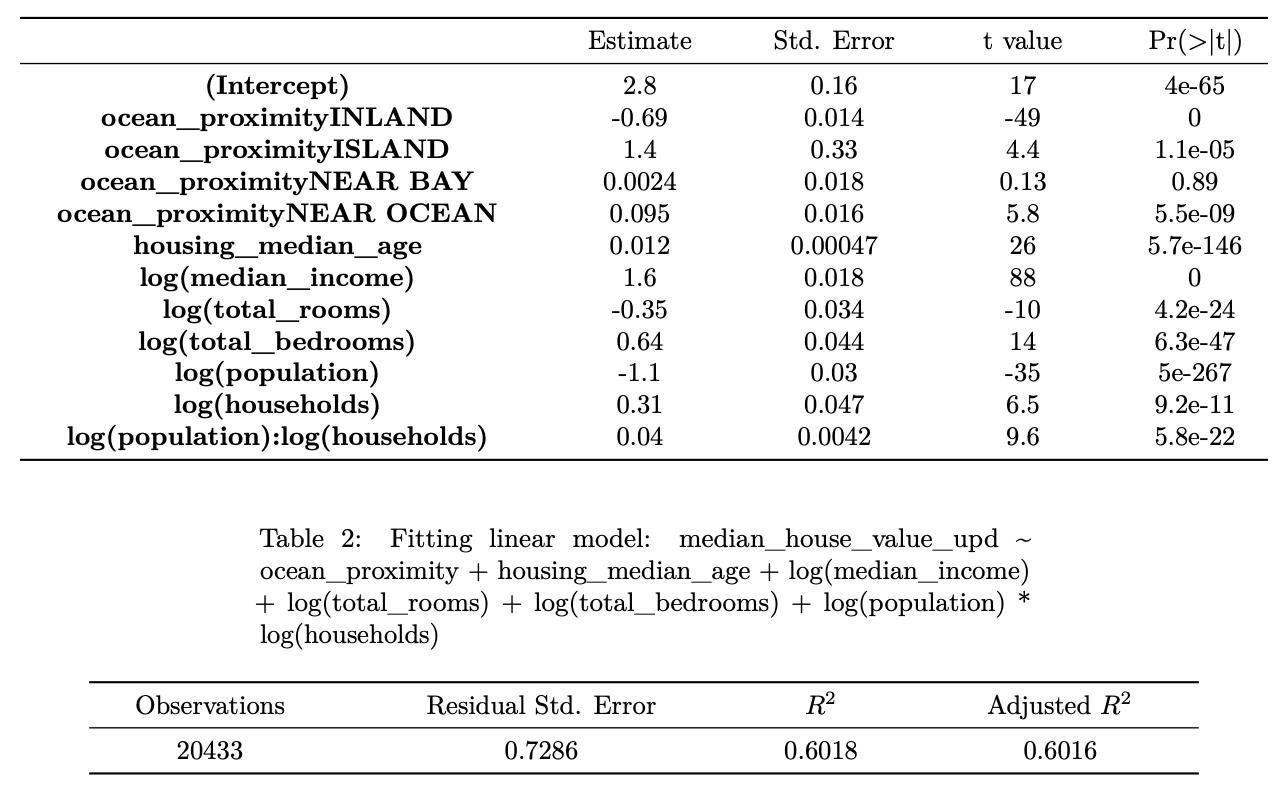
\includegraphics[scale = 0.65]{Regression Table.png}
\end{center}

While the model we developed can be used to estimate the average home prices of homes in the neighborhoods contained in our dataset in 1990, we do not believe that is an appropriate use of the model. Our $R^2$ value (0.60) indicates that our model does not appropriately explain the entire variation in housing prices. Additionally, as we previously noted, we are measuring the mean of median home values so our estimates are likely biased. Thus, using our model to estimate average home prices will not produce reliable estimates. Instead, we think our model should be used to understand the influence that our predictors had on California housing prices in 1990. Because the t-values of our regressors are strong enough, we believe that we have reliable estimates for the effects of the various housing characteristics on housing values despite the risks posed by the omitted variable bias. \\

Our model indicated that ocean proximity had a statistically significant effect on the price of homes. Our reference level is homes less than one hour away from the ocean. The model found that, ceteris paribus, being on an island increased the value of a home compared to living within one hour of the ocean. However, our model found that, all else held equal, homes inland had a lower average value compared to homes within an hour of the ocean. Our model also found that homes near the bay had a marginally higher average value compared to homes within one hour of the ocean. We did not find strong evidence being near the ocean had a statistically significant effect compared to being within one hour of the ocean on home values. \\

Fixing all other variables, homes inland had an average price \$69,000 less than homes within 1 hour of the ocean. We are 95\% confident that the mean prices of homes inland were between \$66,256 and \$71,744 less expensive than those within one hour of the ocean. \\

Homes on an island, on the other hand, had a mean price which was \$140,000 more expensive than those within 1 hour of the ocean, fixing for all other variables. We are 95\% confident that, ceteris paribus, the mean difference in median prices between homes on an island and those within one hour of the ocean was between \$75,320 and \$204,680. \\

Homes that are near the ocean had an average home price \$9,500 more than those within one hour of the ocean after fixing all other variables. We are 95\% confident that, all else held equal, the mean difference between homes near the bay and those within one hour of the ocean was between \$6,364 and \$12,636. \\

The model found a statistically insignificant p-value for the individual t-test of the coefficient on housing prices near the bay compared to within the ocean. Thus, we do not have strong evidence that the prices of homes near the bay were significantly different from those within one hour of the ocean. The boxplot below shows the median housing prices based on ocean proximity. 

\hfill

\begin{center}
    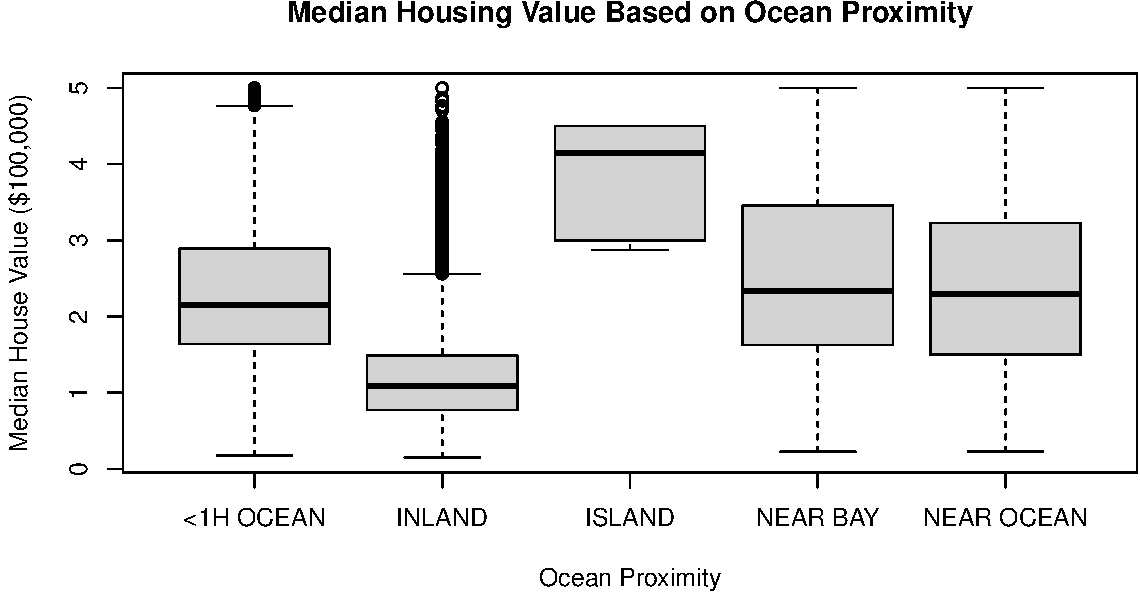
\includegraphics[scale = 0.75]{Median Housing Value (Ocean Proximity).pdf}
\end{center}

\hfill

The boxplot indicates, just as our model suggests, that homes on islands are more expensive. Additionally, we can see that homes near the bay, near the ocean, and within one hour of the ocean all have relatively similar mean values.  Furthermore, inland homes have a lower mean value. Note the large quantity of outliers on the inland boxplot. They can potentially be attributed to factors, like proximity to metropolitan areas and size of homes, that increase the number of outliers inland. There are more homes and more heterogeneity in homes inland compared to those in all other categories—we would be shocked to find a modest starter home on an island. \\

Median home age had a positive effect on housing prices after accounting for all other factors. A one-year increase in median housing age was correlated with an \$1,200 increase in value. We are 95\% confident that, after fixing for all other variables, increasing the age of a home by one year resulted in between a \$1,108 and \$1,292 increase in the mean of its median price. This result is interesting and counterintuitive. \\

The plot below shows the relationship between the median age of a home and its median value in 1990. The plot does not depict a discernible linear relationship. Additionally, there is a large cluster above the median age of 50. We suspect, much like with income, this has to do with an upper bound in census data collection. Then, we hypothesize that many of the most expensive homes in California were built after the gold rush, and thus would qualify as over 50 years old in 1990—potentially causing the regression coefficient on median age to be positive. We do not have sufficient evidence for this claim and further investigation of the data can provide better answers but given the scope of this paper, we are simply positing one possible explanation for a positive coefficient on the median age of a home. 

\hfill

\begin{center}
    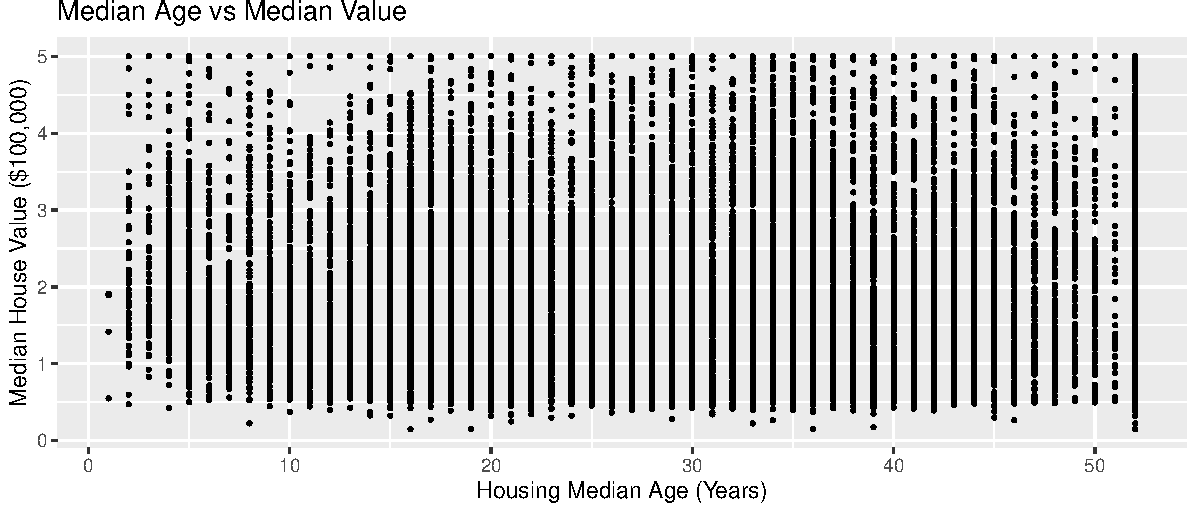
\includegraphics[scale = 0.75]{Median Age vs Median Value.pdf}
\end{center}

Median neighborhood income has a statistically significant effect on mean housing prices. A 10\% increase in median neighborhood income was correlated with a \$15,250 increase in mean housing prices. We are 95\% confident, after fixing for all other variables, that the mean effect fell between a \$15,078 and \$15,421 increase in mean home prices. \\

The below plot depicts the relationship between log(median income) and median home value. The plot depicts a discernible positive linear correlation between the two variables. This makes intuitive sense because, in a block with a higher median income, we expect the homeowners to have purchased more expensive homes.

\hfill

\begin{center}
    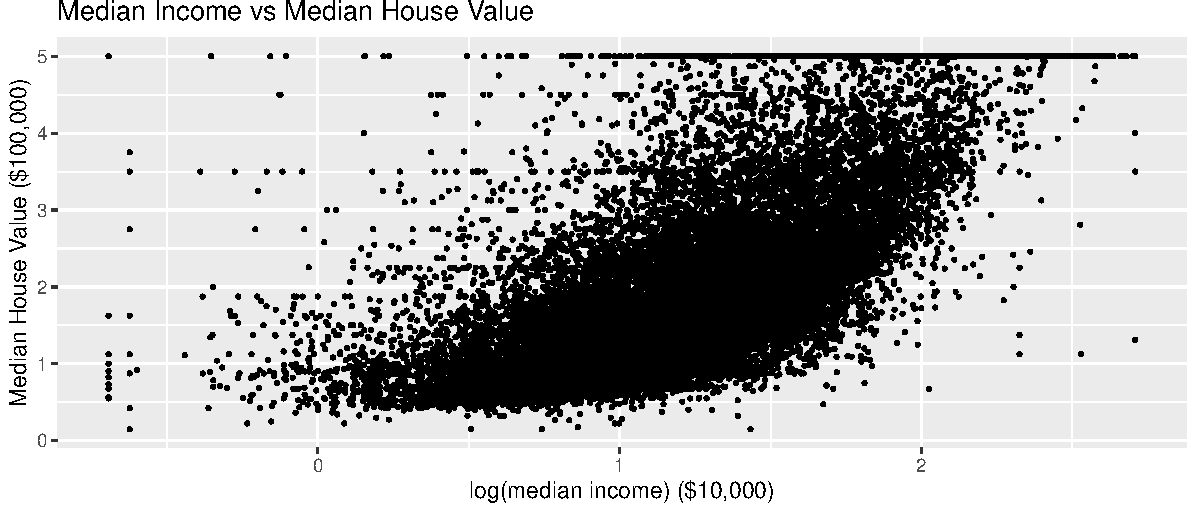
\includegraphics[scale = 0.75]{Median Income vs Median House Value.pdf}
\end{center}

A 10\% increase in total rooms was correlated with between a \$3,012 and \$3,660 decrease in mean housing prices after fixing for all other variables (95\%). The expected change in mean housing prices was a \$3,336 decrease. Unlike the total number of rooms, which decreased the average price, a 10\% increase in the number of \emph{bedrooms} was correlated with between a \$5680 and \$6519 \emph{increase} in housing value after fixing for all other variables (95\%). \\

This result was also counterintuitive. We expected that an increase in total rooms would increase home values because census blocks with many rooms that weren't bedrooms were likely wealthy neighborhoods while census blocks with many \emph{bedrooms} were likely high-density residential areas. One possible explanation is that these high-density residential areas were closer to major cities and thus carried a premium, which is reflected in the coefficients. \\

The below plots show the relationship between log(rooms)and median home values, and log(bedrooms) and median home values. There is clustering between 5 and 10 total log(total rooms) and 4 and 8 log(total bedrooms) but there appears to be a fairly even scatter throughout and no discernible effect between each predictor individually and the response variable, without accounting for the other predictors.

\hfill

\begin{center}
    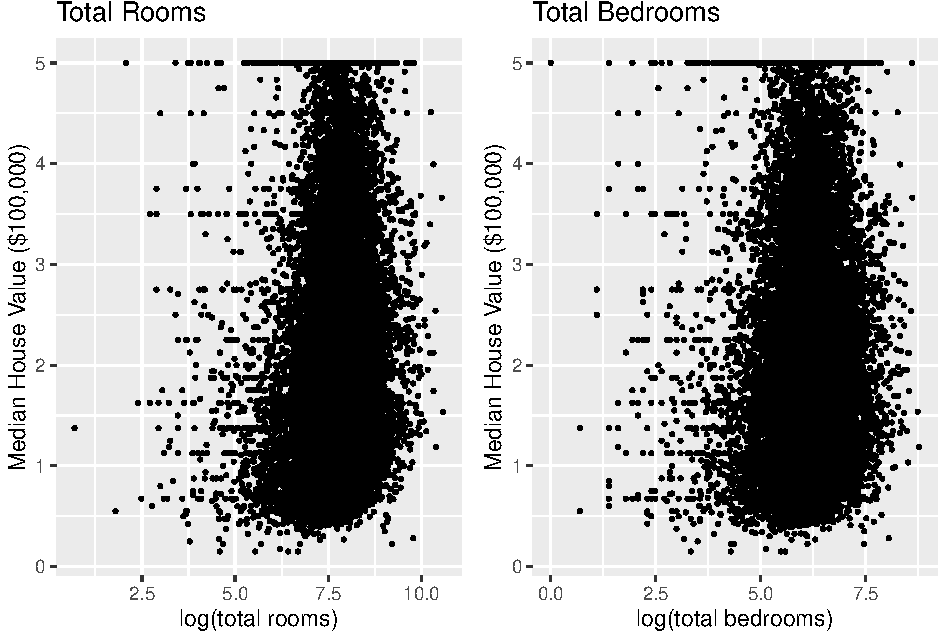
\includegraphics[scale = 0.9]{Total Rooms + Total Bedrooms.pdf}
\end{center}

A 10\% increase in just population, ceteris paribus, was correlated with a \$10,480 decrease in the mean home value. The 95\% confidence interval for that effect went from a decrease of \$10,198 to a decrease of \$10,770. \\ 

A 10\% increase in just the number of households increased the mean home value by \$2,955. The 95\% confidence interval for that effect was \$2,507 to \$3,403. \\

But when there was both a 10\% increase in households and population, the net effect was a decrease in the mean of \$7,148. The 95\% confidence interval for that effect was between a \$6,374 and and \$7,922. This result makes intuitive sense because people value their space so if more households were built within the same block as a home and the population of the block increased as more people move into the block, we would expect the mean home value to decrease. \\

\section*{A brief discussion of our model}

We arrived at our model by beginning with the saturated model and testing all reasonable pairwise correlations. Once we removed all statistically insignificant correlations and determined which coefficients to drop through using AIC and our own logic (such as removing longitude and latitude), we made the necessary transformations to bring all predictor variables to a linear scale. A number of the variables had a fanning out towards the lower end and we applied a log transformation to fix the heteroskedasticity to align the predictor variables with our assumptions for a simple linear regression model. Our final QQ plot can be seen below. There appears to be some heavy-tailed-ness on the right end—which is to be expected with housing prices. We are not concerned by that because of the size of our dataset.

\hfill

\begin{center}
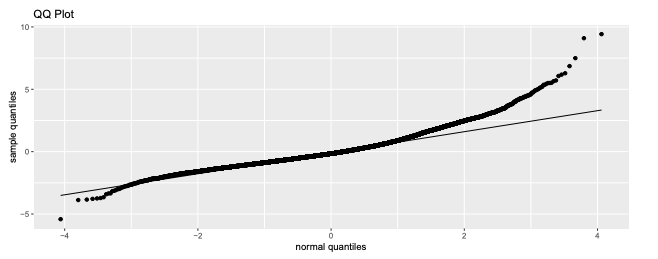
\includegraphics[scale = 0.65]{QQ Plot.png}
\end{center}

\section*{Discussion}

Our multiple regression model found that being on an island, near an ocean, being older, having higher median block group income, and having more total bedrooms in a block group all increased the mean housing prices. Being inland, having more total rooms in a block, and having a higher block group population, all reduced the mean home price. Many of our predictors did not have a clear linear relationship with the response variable without accounting for the other variables. But when compiled, they produced a regression model that can measure their effects on California home values in 1990. \\

The strength of our results and the reliability of our results are constrained by a few important limitations. The first limitation of our model is that we limited ourselves to pairwise interactions and thus were not exhaustive in our analysis of interactions. Furthermore, this data was self-reported in a census from 1990. Our data then is biased by individuals' perceptions of their own home values. Additionally, as we noted earlier, our data only reported the median home values, ages, and block incomes, not the actual home values, ages, and incomes biased our estimates of mean home values, ages, and block incomes. More advanced statistical methods (such as conducting a median regression instead of a mean) might allow us to better examine the effects of these predictors on the data. Additionally, a paper with a larger scope might further investigate some of the coefficient values that surprised us—such as the positive correlation between home age and home value. Additionally, this paper is well suited to an econometric analysis. An econometrician could motivate interactions between variables like total rooms and total bedrooms or total rooms and median block income even if those interactions did not appear statistically significant. \\

Ultimately, this study left us with a number of questions. We remain curious about why there isn't a statistically significant interaction between the total number of bedrooms and the total number of rooms. We remain curious about the inclusion of variables like latitude and longitude which require a background in either GIS or spatial statistics to appropriately evaluate. We remain curious about conducting a time-series analysis of this data to see how the effects of these predictors have changed over time. \\

Our $R^2$ value indicates that only 60\% of the variation in California home prices in 1990 can be explained by our model. Then there is clearly room to include additional variables like proximity to major cities or additional interactions to improve the model. There is a lot to explore when it comes to housing prices, and this model just begins to explore the depth of analysis that one can conduct with more data and a greater knowledge of statistical tools. 

\newpage

\section*{References}

Data Source - https://www.kaggle.com/camnugent/california-housing-prices

Average Housing Price 1990 - https://tinyurl.com/yh2v8ssk


\end{document}
